
%(BEGIN_QUESTION)
% Copyright 2015, Tony R. Kuphaldt, released under the Creative Commons Attribution License (v 1.0)
% This means you may do almost anything with this work of mine, so long as you give me proper credit

Følgende effekt- og tripkretser viser differensialstrømsvern (87) for en stor trefasegenerator:

$$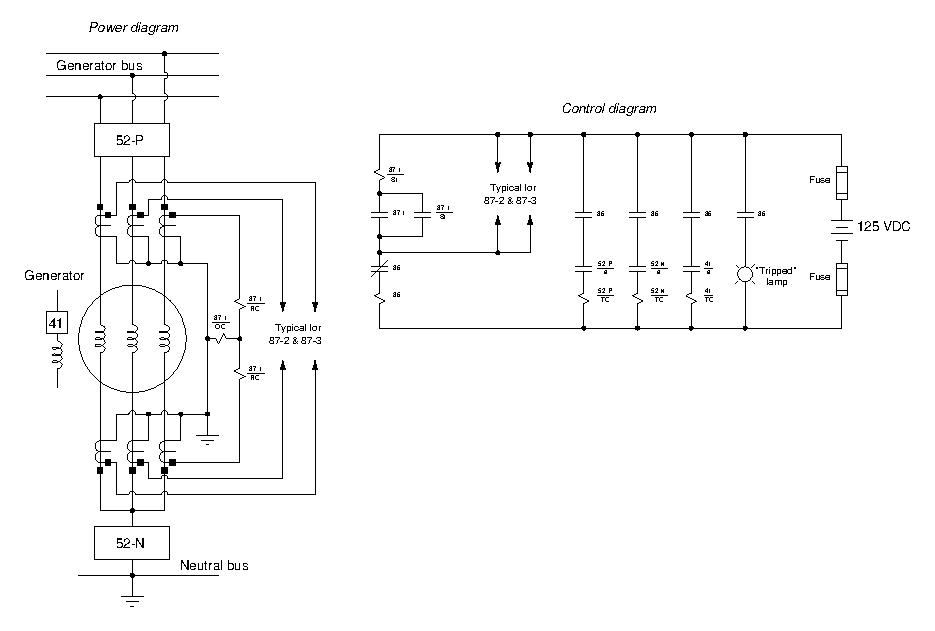
\includegraphics[width=15.5cm]{i01028x01.eps}$$

Anta at relé 87-3 en dag tripper, tripper 86 lockout-reléet og åpner alle tre brytere (52-P, 52-N, 41).

\vskip 10pt

Vurder sannsynligheten for hver angitt feil. Se på én feil om gangen, og avgjør om feilen alene kan forklare {\it alle} målinger og symptomer.

% No blank lines allowed between lines of an \halign structure!
% I use comments (%) instead, so that TeX doesn't choke.

$$\vbox{\offinterlineskip
\halign{\strut
\vrule \quad\hfil # \ \hfil & 
\vrule \quad\hfil # \ \hfil & 
\vrule \quad\hfil # \ \hfil \vrule \cr
\noalign{\hrule}
%
% First row
{\bf Feil} & {\bf Mulig} & {\bf Umulig} \cr
%
\noalign{\hrule}
%
% Another row
DC stasjonsforsyning død &  &  \cr
%
\noalign{\hrule}
%
% Another row
Feil i generator feltvikling &  &  \cr
%
\noalign{\hrule}
%
% Another row
CT feilet åpen &  &  \cr
%
\noalign{\hrule}
%
% Another row
86 tripspole feilet åpen &  &  \cr
%
\noalign{\hrule}
%
% Another row
86 tripspole feilet kortsluttet &  &  \cr
%
\noalign{\hrule}
%
% Another row
87-3/OC-spole feilet åpen &  &  \cr
%
\noalign{\hrule}
%
% Another row
87-3/OC-spole feilet kortsluttet &  &  \cr
%
\noalign{\hrule}
%
% Another row
87-3/RC-spole feilet åpen &  &  \cr
%
\noalign{\hrule}
%
% Another row
87-3/RC-spole feilet kortsluttet &  &  \cr
%
\noalign{\hrule}
} % End of \halign 
}$$ % End of \vbox

\vfil 

\underbar{file i01028}
\eject
%(END_QUESTION)





%(BEGIN_ANSWER)

Dette er en vurderingsoppgave -- ingen fasit eller hint oppgis!

%(END_ANSWER)





%(BEGIN_NOTES)

% No blank lines allowed between lines of an \halign structure!
% I use comments (%) instead, so that TeX doesn't choke.

$$\vbox{\offinterlineskip
\halign{\strut
\vrule \quad\hfil # \ \hfil & 
\vrule \quad\hfil # \ \hfil & 
\vrule \quad\hfil # \ \hfil \vrule \cr
\noalign{\hrule}
%
% First row
{\bf Feil} & {\bf Mulig} & {\bf Umulig} \cr
%
\noalign{\hrule}
%
% Another row
DC stasjonsforsyning død &  & $\surd$ \cr
%
\noalign{\hrule}
%
% Another row
Feil i generator feltvikling &  & $\surd$ \cr
%
\noalign{\hrule}
%
% Another row
CT feilet åpen & $\surd$ &  \cr
%
\noalign{\hrule}
%
% Another row
86 tripspole feilet åpen &  & $\surd$ \cr
%
\noalign{\hrule}
%
% Another row
86 tripspole feilet kortsluttet &  & $\surd$ \cr
%
\noalign{\hrule}
%
% Another row
87-3/OC-spole feilet åpen &  & $\surd$ \cr
%
\noalign{\hrule}
%
% Another row
87-3/OC-spole feilet kortsluttet &  & $\surd$ \cr
%
\noalign{\hrule}
%
% Another row
87-3/RC-spole feilet åpen & $\surd$ &  \cr
%
\noalign{\hrule}
%
% Another row
87-3/RC-spole feilet kortsluttet & $\surd$ &  \cr
%
\noalign{\hrule}
} % End of \halign 
}$$ % End of \vbox


%INDEX% Electric power systems: protective relays (differential)
%INDEX% Electronics review: current transformer (CT)
%INDEX% Protective relay: differential current (87)
%INDEX% Protective relay: troubleshooting

%(END_NOTES)

